\textbf{Beispiel 3}\\ \\
a)\\ \\
Bei dieser RC-Ersatzschaltung wurden die Wärmeübergänge als Widerstände, konstante Temperaturen als Spannungsquellen
und veränderliche Temperaturen als Kapazitäten dargestellt.
\begin{figure}[h]
	\centering
	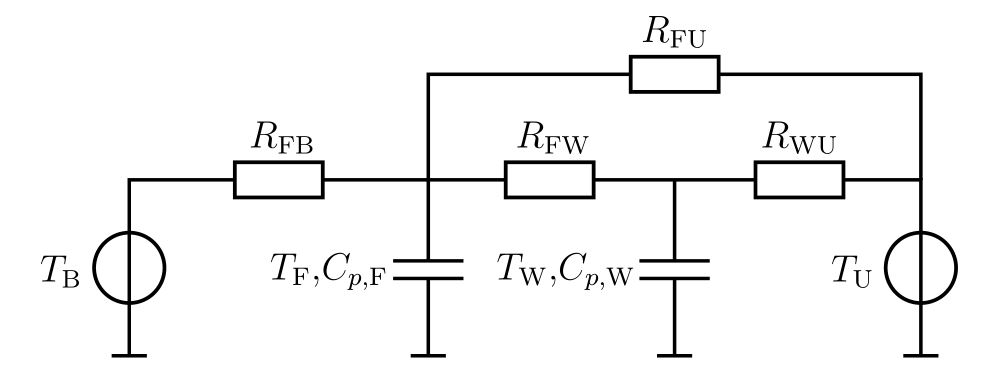
\includegraphics[width= 10cm]{tikz/02_02_2018_3a}
\end{figure}
\newline
b)\\ \\
Aus der RC-Ersatzschaltung ergeben sich folgende Differentialgleichungen
\begin{align*}
	C_{p,F}\frac{\text{d}}{\text{d}t}T_F(t) &= \frac{T_B - T_F(t)}{R_{FB}} + \frac{T_W(t) - T_{F}(t)}{R_{FW}} + \frac{T_U - T_F(t)}{R_{FU}} \\
	C_{p,W}\frac{\text{d}}{\text{d}t}T_W(t) &= \frac{T_U - T_W(t)}{R_{WU}} + \frac{T_F(t) - T_W(t)}{R_{FW}}
\end{align*}
\newpage
\noindent
Im stationären Fall lauten die beiden Differentialgleichungen
\begin{align*}
	0 &= (T_{B,R} - T_{F,R})R_{FW}R_{FU} + (T_{W,R} - T_{F,R})R_{FB}R_{FU} + (T_{U,R} - T_{F,R})R_{FB}R_{FW} \\
	0 &= T_{B,R}R_{FW}R_{FU} + T_{W,R}R_{FB}R_{FU} - T_{F,R}(R_{FW}R_{FU} + R_{FB}R_{FU} + R_{FB}R_{FW}) + T_{U,R}R_{FB}R_{FW}
\end{align*}
und
\begin{align*}
	0 &= (T_{U,R} -  T_{W,R})R_{FW} + (T_{F,R} - T_{W,R})R_{WU} \\
	0&= -T_{W,R}(R_{FW} + R_{WU}) + T_{F,R}R_{WU} + T_{U,R}R_{FW}
\end{align*}
Dadurch erhält man
\begin{align*}
	\textbf{\text{0}} &= \begin{bmatrix}
		R_{FW}R_{FU} & R_{FB}R_{FU} \\
		0 & -R_{FW} - R_{WU}
	\end{bmatrix}
	\begin{bmatrix}
		T_{B,R} \\
		T_{W,R}
	\end{bmatrix} \\
	&-
	\begin{bmatrix}
		R_{FW}R_{FU} + R_{FB}R_{FU} + R_{FB}R_{FW} & -R_{FB}R_{FW} \\
		-R_{WU} & -R_{FW}
	\end{bmatrix}
	\begin{bmatrix}
		T_{F,R} \\
		T_{U,R}
	\end{bmatrix}
\end{align*}
Durch Lösen dieses Gleichungssystem lautet die gesuchte Lösung
\begin{align*}
	T_{B,R} &= \frac{R_{FB}R_{FU} + R_{FB}R_{FW} + R_{FB}R_{WU} + R_{FU}R_{FW} + R_{FU}R_{WU}}{R_{FU}(R_{FW} + R_{WU})}T_{F,R} \\
	&- \frac{R_{FB}R_{FU} + R_{FB}R_{FW} + R_{FB}R_{WU}}{R_{FU}(R_{FW} + R_{WU})}T_{U,R}
\end{align*}